\documentclass[a4paper,12pt,twoside]{book}

\usepackage{praca_dyplomowa}

\author{Michał Sośnicki}
\title{Usprawnienie programowania z użyciem typów w Glasgow Haskell Compiler}

\begin{document}
\frontmatter
\begin{titlepage}
\begin{center}
\textbf{{\large Politechnika Łódzka}\\}
\vspace{\medskipamount}
\textbf{\large Wydział Fizyki Technicznej, Informatyki\\i~Matematyki Stosowanej}
\vspace{\medskipamount}\\
{\large Instytut Informatyki}\\
\vspace{2.5cm}
{\Large Michał Sośnicki\\nr albumu 180692\\}
\vspace{2cm}
{\huge{Usprawnienie programowania z użyciem\\typów w Glasgow Haskell Compiler}}
\end{center}
\vspace{3cm}
\hfill
\begin{minipage}{.55\columnwidth}
Praca inżynierska\\
napisana pod kierunkiem\\
dr inż. Jana Stolarka
\end{minipage}
\vfill
\begin{center}
Łódź 2016
\end{center}
\end{titlepage}

\tableofcontents

\mainmatter
\pagestyle{headings}
\chapter{Wstęp}\label{chap:wstep}

Zakresem niniejszej pracy inżynierskiej jest informatyka, w szczególności tworzenie kompilatorów i systemy typów. Przedmiotem pracy jest usprawnienie programowania z użyciem typów w Glasgow Haskell Compiler.

Wśród popularnych, statycznie typowanych języków istnieje wyraźne rozróżnienie między poziomem typów, a poziomem termów. Zawarte w temacie pracy mechanizmy programowania z użyciem typów służą zatarciu tej granicy. Dają one programistom możliwości wyrażania logiki na poziomie typów przypominające te dostępne na poziomie termów. Gdy zostaną użyte, sprawdzenie typów w trakcie kompilacji może wymagać obliczeń w celu znalezienia typów, do których ewaluują się zapisane na poziomie typów wyrażenia. Zwiększa to precyzję, z jaką możliwe jest opisywanie zachowania programu.

Praca została poświęcona językowi Haskell i kompilatorowi Glasgow Haskell Compiler. Wybór ten został podyktowany dostępnością rozszerzeń umożliwiających programowanie z użyciem typów. GHC oferuje między innymi uogólnione algebraiczne typy danych, promocję typów danych, zależności funkcyjne między parametrami w klasach typów i rodziny typów. Dostępne są również pomocne biblioteki, dostarczające na przykład typ danych Proxy lub pozwalające na promocję zwykłych funkcji do rodzin typów. Szczególnie istotnym rozszerzeniem są rodziny typów, gdyż umożliwiają definiowanie na poziomie typów funkcji wykorzystujących dopasowywanie wzorców oraz zależności funkcyjne, które dają równoważne możliwości, lecz wymagają stosowania stylu relacyjnego zamiast funkcyjnego. Razem zapewniają możliwości zbliżone do tych, które mają języki z typami zależnymi.

Rodziny typów zostały wprowadzone do Haskella w wersji 6.10.1, czyli w roku 2008. Do tej pory są przedmiotem prac naukowych, a ich implementacja jest nieustannie rozwijana. Na przykład w 2015 roku wprowadzone zostały do GHC różnowartościowe rodziny typów. Aktywny rozwój w połączeniu z faktem, iż type checker to największy komponent GHC\cite{AOSA} skutkują tym, iż liczba usprawnień oczekujących na wykonanie jest bardzo duża.

Programowanie z użyciem typów możliwe jest w innych językach. Na przykład, Scala oferuje do tego \foreign{path dependent types}, a w C++ możliwe jest metaprogramowanie z użyciem szablonów. Istnieją też języki z typami zależnymi jak Agda lub Idris. Wiele z tych języków ma implementacje o otwartych źródłach i mogłoby służyć do realizacji tematu pracy zamiast Haskella.

Istnieje kilka implementacji języka Haskell. Spośród nich tylko dwie są zgode z aktualną specyfikacją języka Haskell 2010, Glasgow Haskell Compiler i Utrecht Haskell Compiler\cite{WikiImplementations}. Porównanie repozytoriów pozwala stwierdzić, że spośród nich GHC jest bardziej rozwinięty. Różnica ta objawia się w tym, iż rozszerzenia kompilatora pozwalające na programowanie na poziomie typów jak rodziny typów istnieją wyłącznie w GHC\cite{UHCUserGuide}. Z tego powodu w pracy został wybrany ten kompilator.

\todo[disable,inline]{Wstęp rozprawy powinien jasno określać tematykę i~zakres podejmowanego problemu.
Należy wskazać dlaczego dana tematyka została podjęta. Czy rozwiązania
istniejące w~danej dziedzinie nie są wystarczające? Czy problem można rozwiązać
inaczej? Czy podejmowany problem jest aktywnym tematem badawczym? Przed jakimi
wyzwaniami stoi osoba podejmująca tematykę? Na tym etapie należy zarysować
problem w~sposób ogólny.}

\section{Cele pracy}\label{sec:cele_pracy}

Celem pracy jest dokonanie jak największej liczby usprawnień w kompilatorze GHC. Do organizacji pracy nad kompilatorem wykorzystywany jest system Trac. Przez usprawnienie rozumiane są zmiany w GHC lub w powiązanych z tym projektem bibliotekach, które zostały zgłoszone w systemie Trac. Zatem usprawnienia, tak jak zgłoszenia, mogą polegać na naprawieniu błędu w działaniu kompilatora, zaimplementowaniu nowej funkcjonalności lub wykonaniu pewnego zadania.

W tej pracy podjęte zostały wyłącznie usprawnienia polegające na zmianach w kodzie, w częściach związanych z rozszerzeniami opisanymi powyżej. Wybrane usprawnienia to:

\begin{itemize}
 \item Ujednolicenie wyświetlania rodzin typów w błędach i ostrzeżeniach kompilatora.
 \item Dodanie ostrzeżeń o nieużywanych zmiennych w rodzinach typów.
 \item Naprawienie błędu z niewłaściwym parsowaniem zmiennych zaczynających się od podkreślnika w przypadku kompilacji z rozszerzeniem \code{NamedWildCards}.
\end{itemize}

Poprawne wprowadzenie zmiany w kodzie wymaga przejścia przez procedurę ustaloną przez osoby mające prawa zapisu do repozytorium\cite{WikiFixingBugs}. Zgodnie z nią wykonanie usprawnienia wymaga:

\begin{itemize}
  \item Informowania o stanie pracy w systemie Trac. Oznaczenie swojego konta jako właściciela zadania, uzupełnienie informacji na przykład o testach i powiązanych zadaniach, a na koniec oznaczenie zgłoszenia jako zrealizowanego.
  \item Przygotowania testów pokrywających wprowadzone zmiany. Dodanie ich do zestawu testów wykonywanych w czasie walidacji.
  \item Dokonanie zmian w kodzie w zgodzie z obowiązującymi konwencjami i z dokumentacją. Sporządzenie z nich commitów w systemie kontroli wersji git.
  \item Wysłanie łatki do systemu Phabricator, gdzie przejdzie ona inspekcję. Jeżeli nie będzie ku temu przeszkód, zmiany zostaną przeniesione do głównego repozytorium.
\end{itemize}

\section{Przegląd literatury}\label{sec:przeglad_literatury}

Podstaw teorii budowy kompilatorów dostarcza \cite{Dragon}. Autorzy opisują budowę kompilatora, a następnie każdą fazę kompilacji. Ma to zastosowanie także w przypadku kompilatora GHC. Krótki opis poświęcony konkretnie GHC dostępny jest w \cite{AOSA}. Podstawy teorii typów zawarte są w \cite{TAPL}. Omówiony jest w tej pozycji nietypowany i typowany rachunek lambda i kilka jego wzbogaconych wersji. To bardzo istotne, gdyż pojęcia z rachunku lambda występują powszechnie w dokumentacji, w kodzie GHC i są powszechnie używane w dyskusjach przez programistów. Z drugiej strony część poświęcona podtypowaniu nie ma bezpośredniego zastosowania do GHC oraz opis nie obejmuje typów zależnych. Szczególnie warte uwagi w ramach wprowadzenia teoretycznego są również dwa kursy, dostępne za darmo na platformie Coursera: \foreign{Automata} prowadzony przez Jeffa Ullmana oraz \foreign{Programming Languages} prowadzony przez Dana Grossmana. Są to zaadoptowane do formy kursu internetowego kursy akademickie.

Praca nad GHC wymaga znajomości Haskella, w którym jest tworzony kompilator. \cite{LearnYouAHaskell} i \cite{RealWorldHaskell} stanowią dobre wprowadzenie do tego języka, obie pozycje są dostępne za darmo w Internecie. Z rozszerzeniami zmienionymi w tej pracy, \code{TypeFamilies} i \code{PartialTypeSignatures} można zapoznać się w poradniku użytkownika GHC, w zasobach \cite{GuideTypeFamilies} i \cite{GuidePartialTypeSignatures}.

Strona systemu Trac projektu GHC zawiera wiele zasobów pozwalających zainteresowanym programistą wdrożyć się w projekt. Jest tam między innymi opis jak pobrać i skompilować źródła GHC\cite{WikiNewcomers}, opis procedury wprowadzania zmian w kodzie\cite{WikiFixingBugs} oraz instrukcja konfiguracji i wykorzystania narzędzia Phabricator\cite{WikiPhabricator}.

\todo[disable,inline]{W tym podrozdziale należy szczegółowo uzasadnić dlaczego wybrany został taki
a~nie inny temat pracy. Trzeba przede wszystkim zaprezentować aktualny stan
wiedzy w~danej dziedzinie. Oznacza to konieczność omówienia książek
(ew. artykułów naukowych bądź dokumentacji technicznej) z~których będzie się
korzystać w~trakcie rozprawy. Następnie należy wskazać -- tym razem już
konkretnie -- co nowego zamierza się zrobić. Podstawowymi celami tego
podrozdziału jest wprowadzenie czytelnika w~aktualny stand danej dziedziny
i~przekonanie go że \textbf{naprawdę warto zajmować się podjętym tematem}.}

\section{Układ pracy}\label{sec:uklad_pracy}

Rozdział \ref{chap:wstep} zawiera wprowadzenie i określenie tematu oraz celu pracy. Rozdział \ref{chap:teoria} zawiera opis teorii budowy kompilatorów i systemów typów potrzebnej związanej z tematem. Rozdział \ref{chap:technologie} opisuje technologie i narzędzia wykorzystane w pracy. W rozdziale \ref{chap:badania} przedstawiono opis dokonanych zmian w GHC. Rozdział \ref{chap:podsumowanie} zawiera podsumowanie czy założone cele zostały osiągnięte. Dodatek \ref{app:plyta} zawiera płytę CD z kodem aplikacji\todo{z patchami z moimi zmianami uzyskanymi git diffem?} i kopią tej pracy oraz wykorzystanych źródeł internetowych.

\todo[disable,inline]{Tutaj należy zamieścić opis dalszej zawartości pracy.}

\chapter{Część teoretyczna}\label{chap:teoria}
Ten rozdział powinien zawierać teorię z~której autor będzie korzystał w~dalszej
części pracy.  Podstawowym celem istnieniem tego rozdziału jest umożliwienie
czytelnikowi zrozumienie teorii rozwijanej w pracy oraz osiągniętych wyników
praktycznych.  Jeżeli jakieś informacje nie są niezbędne do zrozumienia
osiągnięć autora nie należy o nich pisać.

\section{Architektura Glasgow Haskell Compiler}
\todo[inline]{Treść. Rysunek z AOSA. Frontend i backed. Opis parser, renamer, type-checker.}

\sectionex{Rodziny typów}{Rozszerzenie TypeFamilies}
\todo[inline]{Treść zaczerpnięta z UsersGuide. Pamiętać o DataFamilies}

\sectionex{Częściowe sygnatury typów}{Rozszerzenie PartialTypeSignatures}
\todo[inline]{Treść zaczerpnięta z UsersGuide. Pamiętać o NamedWildCards}

\chapter{Użyte narzędzia i~technologie}\label{chap:technologie}

\section{Język programowania}\label{sec:jezyk_programowania}

Glasgow Haskell Compiler został napisany w~języku Haskell. Wykorzystano została
w~projekcie technika \foreign{bootstraping}, polegająca na tym, iż kompilator
rozwijany jest w~języku, który kompiluje i~jedną z~zależności potrzebną do
zbudowania GHC jest on sam. Środowiskiem wykorzystanym do edycji kodu było
IntelliJ IDEA z~wtyczką zapewniającą wsparcie dla języka Haskell. Wtyczka ta
niestety w~pełni działa tylko z~projektami systemu Cabal i~nie jest dostosowana
do prac nad GHC. Z~tego powodu środowisko nie zapewniało na przykład ciągłego
raportowania błędów w~kodzie lub wyszukiwania deklaracji określonego typu, choć
z~tych udogodnień można korzystać w~innych projektach.

Testowanie i~walidacja kompilatora są realizowane przez skrypty w~języku
Python. Jest on wymagany do zbudowania GHC
również z~tego powodu, że do stworzenia dokumentacji wykorzystane zostało
narzędzie Sphinx, wymagające interpretera.

W~projekcie użyty został również język C do napisania środowiska
uruchomieniowego, linkowanego z~każdym programem skompilowanym przez GHC.
W~pozostałych częściach GHC można znaleźć dyrektywy preprocesora C, który GHC może
wykorzystać zanim przejdzie do kompilacji. W~tej pracy jednak kontakt z~nim był
znikomy.

\section{Narzędzia}

\subsection{Git}

Kod GHC znajduje się w~repozytorium Git i~jest publicznie dostępny do
pobrania pod adresem \url{http://git.haskell.org/ghc.git}.
Biblioteki wykorzystywane w~kompilatorze również są przechowywane
w~repozytoriach Gita, lecz są osobnymi projektami, dołączonymi do GHC jako
submoduły. Klon oficjalnego repozytorium znajduje się również w~popularnym
serwisie GitHub. Prawa zapisu do repozytorium są
ograniczone\cite{WikiGettingTheSources}.

Krokiem wymaganym do rozpoczęcia pracy było sklonowanie repozytorium i~lokalne
zbudowanie kompilatora ze źródeł. Po lokalnej edycji plików zmiany musiały
zostać zapisane w~repozytorium i~opatrzone komentarzem stosującym się do
konwencji opisanej na wiki GHC, zanim mogły zostać wysłane z~użyciem systemu
Phabricator.

\subsection{Trac}

Trac to system do organizacji pracy programistów. Przechowuje listę zgłoszeń,
czyli spójnych propozycji zmian w~projekcie. Zapisywane są w~nim zadania do
wykonania oraz błędy wykryte w~GHC, także przez zwykłych użytkowników. Chroni to
je przed zapomnieniem w~razie, gdyby nie było możliwe zajęcie się nimi od
razu. Znajdują się w~tym systemie również propozycje dodania nowych funkcji. Do
każdego zgłoszenia może być dołączony opis, w~przypadku błędu sposób
reprodukcji, zapewnione jest miejsce na dyskusję i~mechanizm śledzenia stanu
wykonania zadania. Aby ułatwić organizację pracy, możliwe jest przypisanie do zgłoszeń
właściciela, by zapobiec sytuacji, w~której tę samą rzecz wykonuje
wiele osób. Możliwe jest określenie priorytetu i~planowanej wersji, w~której
zadanie powinno już być wykonane i~późniejsze sprawdzanie, czy ten cel został
osiągnięty. Ułatwione jest również umieszczanie odnośników do innych,
powiązanych zgłoszeń czy do systemu Phabricator. Wszystkie te funkcje
wykorzystywane są w~GHC.

\begin{figure}[ht]
    \centering
    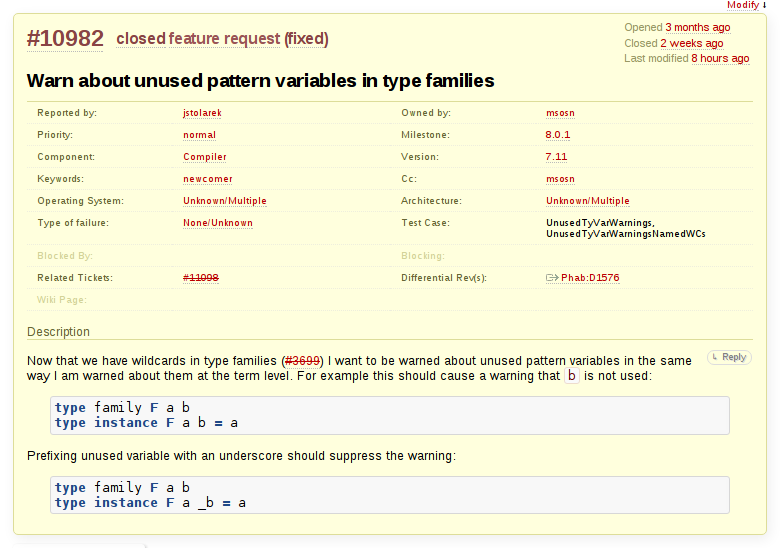
\includegraphics[width=0.8\textwidth]{images/Trac_description}
    \caption{Opis zgłoszenia w systemie Trac}
    \label{fig:Trac_description}
\end{figure}

Przykład zgłoszenia widoczny jest na rysunku \ref{fig:Trac_description}. Dotyczy
ono jednego z~wykonanych w~pracy usprawnień, pozostałe również mają swoje opisy
w~systemie. Aktualizacja informacji na stronie Trac jest wymagana przez
procedurę wprowadzania zmian w~GHC\cite{WikiFixingBugs}.

\subsection{Phabricator}

\cite{WikiPhabricator}

Phabricator wykorzystywany jest do inspekcji kodu w~czasie zgłaszania ulepszenia
oraz do automatycznej walidacji z~wykorzystaniem narzędzia
Harbormaster. Inspekcja jest ułatwiona, gdyż program prezentuje obok siebie
wersję sprzed i~po dokonaniu zmian, z~wyróżnieniem zmodyfikowanych linii
kodu. Daje też możliwość komentowania wybranych fragmentów.

\begin{figure}[ht]
    \centering
    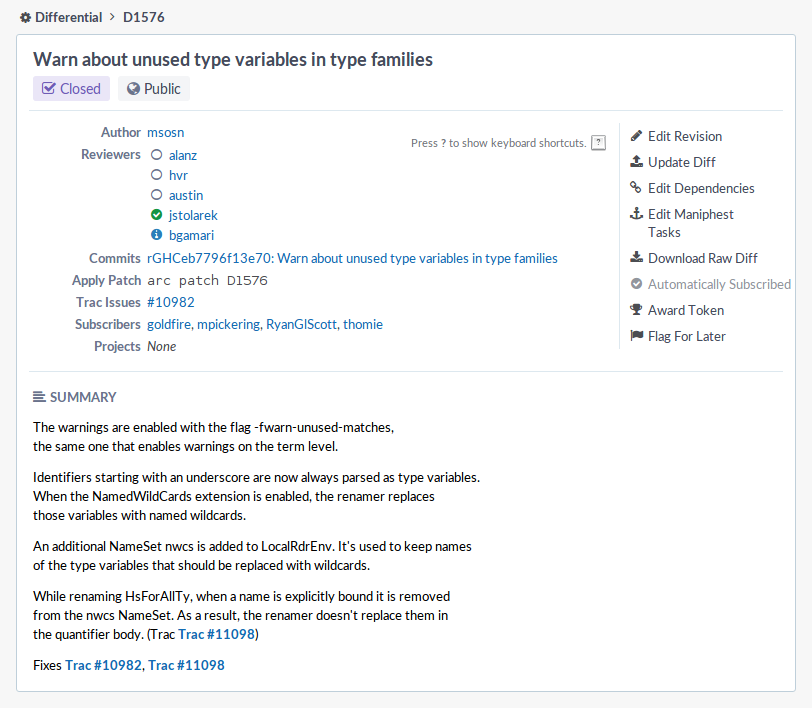
\includegraphics[width=0.8\textwidth]{images/Phabricator_summary}
    \caption{Informacje o proponowanej zmianie w kodzie na stronie Phabricator}
    \label{fig:Phabricator_summary}
\end{figure}

Na rysunku \ref{fig:Phabricator_summary} widać opis jednego z~ulepszeń
dokonanego w~tej pracy. Zgodnie z~procedurą \cite{WikiFixingBugs}, aby zmiany
zapisane w~lokalnym repozytorium Git znalazły się na serwerze, łatka musi
przejść wpierw przez proces rewizji w~systemie Phabricator. Polega on na tym, iż
inni programiści, szczególnie ci, którzy posiadają uprawnienia do zapisu do
repozytorium, zapoznają się z~przesłanym kodem. Zgłaszają oni swoje uwagi
i~decydują, czy zmiana może zostać naniesiona na repozytorium na serwerze, czy
wymaga poprawek.

\begin{figure}[ht]
    \centering
    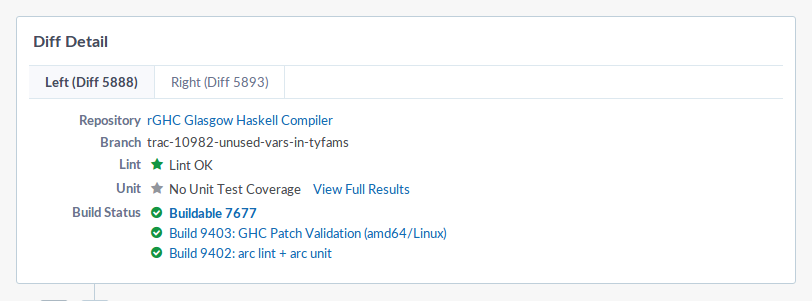
\includegraphics[width=0.9\textwidth]{images/Phabricator_validate}
    \caption{Wynik walidacji programu Harbormaster widoczny na stronie Phabricator}
    \label{fig:Phabricator_validate}
\end{figure}

Z~chwilą wysłania proponowanych zmian w~kodzie do Phabricatora, wykonane zostaje
również automatyczne zbudowanie i~przetestowanie nowej wersji GHC przez moduł
Harbormaster na przeznaczonym do tego serwerze. Jeżeli walidacja wykryje błędy,
jest to znak, iż konieczne są poprawki i~oszczędza to czas poświęcony na
inspekcję kodu przez programistów. Na rysunku \ref{fig:Phabricator_validate}
widać raport z~Harbormastera do jednego z~wprowadzonych w~tej pracy usprawnień,
w~którym nie wykryto problemów.

Jak wspomniane zostało w~sekcji \ref{sec:jezyk_programowania}, GHC jest budowany
z~użyciem innej wersji GHC. Aby zapewnić stabilność, istnieje wymaganie, że nowa
wersja kompilatora musi być możliwa do skompilowania z~wykorzystaniem dowolnej
z~dwóch poprzednich stabilnych wersji\cite{WikiFixingBugs}. Sam proces budowania
przebiega wieloetapowo. Najpierw, z~użyciem starszej wersji kompilatora,
budowane są biblioteki, zależności GHC. Następnie kompilowany w~ten sposób jest
sam GHC, czego rezultatem jest kompilator w~nowszej wersji. Następnie te dwa
kroki, budowania bibliotek i~kompilacji GHC, są powtarzane, lecz
z~wykorzystaniem nowego kompilatora i~to on jest uznawany za wynik całego
procesu\cite{WikiBuildSystem}. Dzięki temu sposobowi działania, usprawnienia
w~kompilacji są od razu zastosowane do kompilatora, przy jednym etapie
wykorzystywane byłyby optymalizacje i~sposób generowania kodu ze starszej
wersji. Stanowi to również dobry test nowej wersji, gdyż jeżeli pojawiły się
w~niej nowe błędy, to jest duża szansa, iż ujawnią się one w~czasie budowania
kompilatora na drugim etapie.

Uzyskany kompilator jest poddawany kilku tysiącom testów. W~większości dzielą
się one na trzy kategorie: testów, w~których kompilacja pewnego programu musi
zakończyć się powodzeniem; testów, których kompilacja musi zakończyć się błędem;
testów, w~których kompilacja musi się udać, a~następnie sprawdzane jest
zachowanie programu po uruchomieniu. Wiele testów polega na sprawdzeniu
komunikatów kompilatora i~porównaniu ze wzorcem.

\chapter{Usprawnienia Glasgow Haskell Compiler}\label{chap:badania}
\todo[disable,inline,size=\tiny]{Ten rozdział zawiera opis wyników uzyskanych w~ramach pracy. Jeśli praca miała
cel badawczy należy skupić się na opisie przeprowadzonych eksperymentów oraz
prezentacji i~analizie uzyskanych wyników. Jeśli praca nie miała na celu
uzyskania nowatorskich wyników, należy skupić się na opisie architektury
stworzonej aplikacji. W~obu przypadkach podstawowym celem tego rozdziału jest
realizacja celów postawionych w~rozdziale \ref{sec:cele_pracy}. Rozdział ten ma
bezspornie pokazywać, że cele pracy zostały zrealizowane}

\sectionex{Zgłoszenie nr 10839}{Consistent pretty-printing of type families}
\label{sec:zgloszenie_10839}

Pierwszym z wykonanych w pracy usprawnień było ujednolicenie wyświetlania rodzin typów. Problem polegał na tym, iż w zależności od miejsca i rodzaju błędu, wyświetlane były one w różny sposób. Co gorsza, różniły się one nie tylko formatem, ale też tym, które informacje zawierają. Widać to na poniższych wycinkach z komunikatów generowanych przez kompilator. We fragmencie \ref{lst:consistent_conflicting_before} z błędem w otwartej rodzinie typów widoczna jest lewa strona równań i wskazania, w którym miejscu w pliku się one znajdują.

\begin{lstlisting}[float,numbers=left,firstnumber=4,label={lst:consistent_conflicting_code},
                   caption={Fragment testu T7524 z dwoma równaniami otwartej rodziny typów będącymi w konflikcie.}]
type family F (a :: k1) (b :: k2)
type instance F a a = Int
type instance F a b = Bool
\end{lstlisting}

\begin{lstlisting}[float,language={},label={lst:consistent_conflicting_before},
                   caption={Błąd generowany przez kompilator w przypadku \ref{lst:consistent_conflicting_code} przed wprowadzeniem zmian.}]
T7524.hs:5:15:
    Conflicting family instance declarations:
      F a a -- Defined at T7524.hs:5:15
      F a b -- Defined at T7524.hs:6:15
\end{lstlisting}

We fragmencie \ref{lst:consistent_overlapped_before} z zamkniętą rodziną typów widoczna jest zarówno lewa jak i prawa strona równania. Nie jest jednak podane miejsce wystąpienia.

\begin{lstlisting}[float,numbers=left,firstnumber=70,label={lst:consistent_overlapped_code},
                   caption={Fragment testu T6018 z zamkniętą rodziną typów z równaniami o nachodzących na siebie dziedzinach.}]
-- This is similar, except that the last equation contains concrete type.  Since
-- it is overlapped it should be dropped with a warning
type family Foo a = r | r -> a where
    Foo Int  = Bool
    Foo Bool = Int
    Foo Bool = Bool
\end{lstlisting}

\begin{lstlisting}[float,language={},label={lst:consistent_overlapped_before},
                   caption={Ostrzeżenie generowane przez kompilator w przypadku \ref{lst:consistent_overlapped_code} przed wprowadzeniem zmian.}]
T6018.hs:75:5: Warning:
    Type family instance equation is overlapped:
      Foo Bool = Bool
\end{lstlisting}

W \ref{lst:consistent_injectivity_before} wyświetlany jest kwantyfikator wiążący zmienne równania i obie strony równania, ale brak jest wcięcia, przez co równanie jest wyrównanie w pionie z resztą komunikatu i cierpi czytelność komunikatu. Brak jest również lokalizacji.

\begin{lstlisting}[float,numbers=left,firstnumber=64,label={lst:consistent_injectivity_code},
                   caption={Fragment testu T6018fail z równaniem rodziny typów nie spełniającej warunku różnowartościowości.}]
-- This should fail because there is no way to determine k from the RHS
type family Fc (a :: k) (b :: k) = r | r -> k
type instance Fc a b = Int
\end{lstlisting}

\begin{lstlisting}[float,language={},label={lst:consistent_injectivity_before},
                   caption={Błąd generowany przez kompilator w przypadku \ref{lst:consistent_injectivity_code} przed wprowadzeniem zmian.}]
T6018fail.hs:66:15: error:
    Type family equation violates injectivity annotation.
    Kind variable ‘k’ cannot be inferred from the right-hand side.
    (enabling -fprint-explicit-kinds might help)
    In the type family equation:
    forall (k :: BOX) (a :: k) (b :: k). Fc a b = Int
\end{lstlisting}


\subsection{Rozwiązanie} %%%

Po zapoznaniu się z kod GHC, udało się odnaleźć miejsca odpowiadające za każdy z tych komunikatów. Są to odpowiednio funkcja \code{inaccessibleCoAxBranch} dla \ref{lst:consistent_overlapped_before}, \code{pprCoAxBranch} w przypadku \ref{lst:consistent_injectivity_before} i \code{pprCoAxBranchHdr} w przypadku \ref{lst:consistent_conflicting_before}. Znaleziono jeszcze inną funkcję \code{pprCoAxiom}, używaną do generowania komunikatów przy kompilacji z flagą \code{-ddump-types}. Wszystkie one służyły do prezentowania rodzin typów w komunikatach, lecz były zaimplementowane osobno. Stąd nietrudno było o rozbieżności.

Dokonano usprawnienia, które polegało na zrefaktorowaniu kodu i wydzieleniu części wspólnej do osobnej funkcji \code{ppr\_co\_ax\_branch}. Została ona napisana tak, by wyświetlać wszystkie informacje, które wydobywały zastąpione funkcje. W komunikacie znajduje się zatem jawny kwantyfikator, wyświetlany tylko przy kompilacji z odpowiednią flagą lub jeżeli rodzina typów wykorzystuje polimorfizm na poziomie rodzajów jak w przykładzie \ref{lst:consistent_injectivity_before}, obie strony równania i miejsce wystąpienia w kodzie kompilowanego programu.

W trakcie pracy okazało się, że rodziny typów danych wymagają innego sposobu wyświetlania prawej strony równania. Jest tak, gdyż ich reprezentacja na etapie sprawdzania typów zawiera wygenerowany przez kompilator konstruktor typu, o którym użytkownik może nie wiedzieć. Z tego powodu \code{pprCoAxBranch} używa funkcji \code{pprDataCons}, która wydobywa z tego wewnętrznego konstruktora typu konstruktory wartości i odtwarza prawą stronę równania taką, jaką podał użytkownik. Przykład działania widoczny jest we fragmencie \ref{lst:consistent_datafams_after}. Wcześniej prawa strona nie była wcale w tym przypadku wcale wyświetlana, co widać na wycinku \ref{lst:consistent_datafams_before}.

\begin{lstlisting}[float,numbers=left,firstnumber=13,label={lst:consistent_datafams_code},
                   caption={Fragment testu T9371 z rodziną typów danych powiązaną z klasą \code{C} i równaniami o nachodzących na siebie dziedzinach.}]
instance {-# OVERLAPPABLE #-} Monoid x => C x where
    data D x = D1 (Either x ())
    makeD = D1 (Left mempty)

instance (Monoid x, Monoid y) => C (x, y) where
    data D (x,y) = D2 (x,y)
    makeD = D2 (mempty, mempty)
\end{lstlisting}

\begin{lstlisting}[float,language={},label={lst:consistent_datafams_before},
                   caption={Błąd generowany przez kompilator w przypadku \ref{lst:consistent_datafams_before} przed wprowadzeniem zmian.}]
T9371.hs:14:10:
    Conflicting family instance declarations:
      D -- Defined at T9371.hs:14:10
      D (x, y) -- Defined at T9371.hs:18:10
\end{lstlisting}

\begin{lstlisting}[float,language={},label={lst:consistent_datafams_after},
                   caption={Błąd generowany przez kompilator w przypadku \ref{lst:consistent_datafams_after} przed wprowadzeniem zmian.}]
T9371.hs:14:10:
    Conflicting family instance declarations:
      D = D1 (Either x ()) -- Defined at T9371.hs:14:10
      D (x, y) = D2 (x, y) -- Defined at T9371.hs:18:10
\end{lstlisting}

Inaczej wygląda to w przypadku funkcji \code{pprCoAxiom}, która jest używana przy generowaniu zrzutu z type-checkera przy kompilacji z odpowiednią flagą. Tutaj pożądane jest wyświetlenie wewnętrznej reprezentacji i \code{pprDataCons} nie jest używana. Przykładowy efekt widać na przykładzie \ref{lst:consistent_tcdump}.

\begin{lstlisting}[float,language={},label={lst:consistent_tcdump},
                   caption={Fragment oczekiwanego zrzutu z type-checkera testu DataFamilyInstanceLHS z wyświetlonym równaniem rodziny typów danych.}]
COERCION AXIOMS
  axiom DataFamilyInstanceLHS.TFCo:R:SingMyKind_ ::
    Sing = DataFamilyInstanceLHS.R:SingMyKind_
      -- Defined at DataFamilyInstanceLHS.hs:8:15
\end{lstlisting}

Przy okazji tego zadania wprowadzony został również drobny refaktoring polegający na wprowadzeniu osobnej funkcji \code{vbar} reprezentującej komunikat \code{"|"}. Definiowane wcześniej lokalnie wystąpienia tego komunikatu zostały zastąpione.

\subsection{Testy} %%%

Do tego zadania nie zostały utworzone nowe testy. Jako że wprowadzona zmiana dotyczyła komunikatów o błędach, istniejące już testy pokrywały ją w wystarczającym stopniu. Dwadzieścia dziewięć testów wykazało wprowadzone przy tym zgłoszeniu zmiany i zostały uaktualnione, by oczekiwać nowych komunikatów. Fragmenty testów \ref{lst:consistent_conflicting_code}, \ref{lst:consistent_injectivity_code} i \ref{lst:consistent_overlapped_code} zaprezentowane wcześniej również wywołały inne komunikaty, które przedstawiono na wycinkach \ref{lst:consistent_conflicting_code}, \ref{lst:consistent_injectivity_code} i \ref{lst:consistent_overlapped_code}.

\begin{lstlisting}[float,language={},label={lst:consistent_conflicting_after},
                   caption={Błąd generowany przez kompilator w przypadku \ref{lst:consistent_conflicting_code} po wprowadzeniu zmian.}]
T7524.hs:5:15:
    Conflicting family instance declarations:
      forall (k :: BOX) (a :: k). F a a = Int -- Defined at T7524.hs:5:15
      forall (k :: BOX) (k1 :: BOX) (a :: k) (b :: k1).
        F a b = Bool -- Defined at T7524.hs:6:15
\end{lstlisting}

\begin{lstlisting}[float,language={},label={lst:consistent_overlapped_after},
                   caption={Ostrzeżenie generowane przez kompilator w przypadku \ref{lst:consistent_overlapped_code} po wprowadzeniu zmian.}]
T6018.hs:75:5: Warning:
    Type family instance equation is overlapped:
      Foo Bool = Bool -- Defined at T6018.hs:75:5
\end{lstlisting}

\begin{lstlisting}[float,language={},label={lst:consistent_injectivity_after},
                   caption={Błąd generowany przez kompilator w przypadku \ref{lst:consistent_injectivity_code} po wprowadzeniu zmian.}]
T6018fail.hs:66:15: error:
    Type family equation violates injectivity annotation.
    Kind variable ‘k’ cannot be inferred from the right-hand side.
    (enabling -fprint-explicit-kinds might help)
    In the type family equation:
      forall (k :: BOX) (a :: k) (b :: k).
        Fc a b = Int -- Defined at T6018fail.hs:66:15
\end{lstlisting}

Wszystkie trzy komunikaty mają ten sam format. Zawierają obie strony równania i lokalizację oraz takie same wcięcia, wyróżniające je od pozostałej części błędu. Dwa fragmenty, w których użyta została zmienna \code{k} są wyświetlane z kwantyfikatorem, choć wcześniej w przypadku \ref{lst:consistent_conflicting_code} informacja o polimorfizmie na poziomie rodzajów typów była niewidoczna.


\sectionex{Zgłoszenie nr 10982}{Warn about unused pattern variables in type families}
\label{sec:zgloszenie_10982}

Zgłoszenie to polegało na dodaniu ostrzeżeń o nieużywanych zmiennych w funkcjach na poziomie typu, działających analogicznie do obecnych już w GHC ostrzeżeń w funkcjach na poziomie termów. Są one uaktywniane tą samą flagą \code{-fwarn-unused-matches}, domyślnie nie są wyświetlane.

Ważnym zagadnieniem okazało się zdefiniowanie, kiedy zmienna typu uważana jest za używaną. W zaimplementowanej wersji, by ostrzeżenie nie było generowane, zmienna musi występować po prawej stronie równania lub występować przynajmniej dwa razy po lewej stronie równania. Obie sytuacje są pokazane we fragmencie \ref{lst:unused_used_examples}

\begin{lstlisting}[float,label={lst:unused_used_examples},
                   caption={Przykład funkcji na poziomie typów ze zmiennymi uznawanymi za wykorzystywane.}]
type family X a where
  X a = a

type family Y a b where
  Y a a = Int
\end{lstlisting}

Aby ostrzeżenie nie wystąpiło, gdy zmienna jest nieużywana, należy zastąpić ją lub poprzedzić podkreślnikiem. Pokazane to zostało we fragmencie \ref{lst:unused_underscore_examples}.

\begin{lstlisting}[float,label={lst:unused_underscore_examples},
                   caption={Przykład funkcji na poziomie typów ze zmiennymi zastąpionymi lub poprzedzonymi podkreślnikami.}]
type family D a b where
  D a _b = a

type family E a b where
  E a _ = a
\end{lstlisting}

\subsection{Rozwiązanie} %%%

Wyświetlania ostrzeżeń dokonano przez zmiany w renamerze. Po analizie kodu udało się stwierdzić, że funkcja \code{rnFamInstDecl} odpowiada za wszystkie rodziny typów w kodzie, otwarte, zamknięte i związane z klasą. Ponadto jest już w niej używana funkcja \code{extractHsTysRdrTyVars}, która przechodzi po typie, kolekcjonując nazwy zmiennych, by utworzyć z nich zmienne typów. Zbiór zmiennych używanych to z kolei to samo, co zbiór zmiennych wolnych w prawej stronie równania, zwracany przez funkcję \code{rnPayload}. Większość informacji potrzebnych do realizacji założeń zgłoszenia było zatem dostępnych od początku, potrzebne było pozyskanie informacji o duplikatach.

W tym celu zastąpiona funkcja \code{extractHsTysRdrTyVars} zastąpiona została bardzo podobną \code{extractHsTysRdrTyVarsDups}, która zwraca wszystkie wystąpienia zmiennych z typu, nie usuwając wielokrotnych wystąpień tej samej nazwy. To umożliwiło sprawdzanie drugiego z warunków, kiedy zmienna jest uznawana za używaną.

Do wygenerowania ostrzeżeń użyta została funkcja \code{warnUnusedMatches}, ta sama, która odpowiada za ostrzeżenia w funkcjach na poziomie termów. Gwarantuje to, że ostrzeżenia te są w tym samym formacie. Następuje w niej również odczytanie ze środowiska globalnego w monadzie renamera, czy opcja generowania ostrzeżeń została wybrana przez programistę, na przykład przez ustawienie flagi \code{-fwarn-unused-matches} lub \code{-Wall}.

Ignorowanie zmiennych zaczynających się od podkreślnika zachodzi w \code{warnUnusedMatches} przez zwyczajne sprawdzenie pierwszego znaku nazwy. Z kolei anonimowe i nazwane symbole wieloznaczne nie wywołują ostrzeżeń, gdyż nie są kolekcjonowane w funkcji \code{extractHsTysRdrTyVarsDups}, więc wcale nie znajdują się na liście nazw.

Zmiana wymagała przejrzenia rodzin typów w GHC oraz powiązanych bibliotekach i uaktualnienia ich tak, by nie generowały ostrzeżeń. W przeciwnym proces walidacji kończyłby się błędem, gdyż został on skonfigurowany, by nie dopuszczać ostrzeżeń w pewnych częściach projektu. Z tego powodu konieczne było stworzenie niewielkiej łatki do biblioteki Hoopl, w której poprzedzono problematyczne zmienne podkreślnikami. Bez żadnych przeszkód znalazła się ona w repozytorium tego projektu.

\subsection{Testy} %%%

Testami sprawdzającymi działanie usprawnienia są \code{UnusedTyVarWarnings} i \code{UnusedTyVarWarningsNamedWCs}. Oba działają przez próbę kompilacji pewnego programu i sprawdzenie, czy na wyjściu kompilatora pojawiają się oczekiwane ostrzeżenia. Program ten zawiera jedenaście przykładów rodzin typów otwartych, zamkniętych lub rodzin typów danych. Spośród ich równań są przypadki zmiennych nieużywanych, używanych ze względu na wystąpienie po prawej stronie i używanych ze względu na wielokrotne wystąpienie po lewej stronie, z nazwą poprzedzoną podkreślnikiem oraz symboli wieloznacznych. Testy te różnią się od siebie tym, iż w przypadku \code{UnusedTyVarWarningsNamedWCs} kompilacja zachodzi z uaktywnionym rozszerzeniem \code{NamedWildCards}. Ma to związek ze zgłoszeniem opisanym w sekcji \ref{sec:zgloszenie_11098}

Fragment \ref{lst:unused_test_code} to część jednego z opisanych testów. Z kolei fragment \ref{lst:unused_test_stderr} to ostrzeżenia, które są dla niego oczekiwane.
\begin{lstlisting}[float,numbers=left,firstnumber=7,label={lst:unused_test_code},
                   caption={Fragment testu \code{UnusedTyVarWarnings} z równaniami wywołującymi ostrzeżenia lub zawierającymi zmienne poprzedzone podkreślnikiem.}]
type family C a b where
  C a b = a                 -- should warn

type family C2 a b
type instance C2 a b = a    -- should warn

type family D a b where
  D a _b = a                -- should not warn

type family D2 a b
type instance D2 a _b = a   -- should not warn
\end{lstlisting}

\begin{lstlisting}[float,language={},label={lst:unused_test_stderr},
                   caption={Ostrzeżenia generowany przez kompilator dla fragmentu \ref{lst:unused_test_code} po wprowadzeniu zmian.}]
UnusedTyVarWarnings.hs:8:5: warning:
    Defined but not used: type variable ‘b’

UnusedTyVarWarnings.hs:11:18: warning:
    Defined but not used: type variable ‘b’
\end{lstlisting}

Dodanie nowej funkcji wymagało jeszcze uaktualnienia dokumentacji. Informacje o dodanych ostrzeżeniach zostały dodane do przewodnika użytkownika w części z opisem opcjonalnych ostrzeżeń, w części z opisem rodzin typów i do dziennika zmian,


\sectionex{Zgłoszenie nr 11098}{PartialTypeSignatures mishandles type variables that begin with an underscore}
\label{sec:zgloszenie_11098}

W tym zgłoszeniu konieczne było naprawienie błędu związanego z rozszerzeniem \code{NamedWildCards}. Problem ten napotkany został w czasie pracy nad zgłoszeniem nr 10982 opisanym w sekcji \ref{sec:zgloszenie_10982}, gdy zbadano jak uaktywnienie tego rozszerzenia wpływa na nazwane symbole wieloznaczne w rodzinach typów. Stąd został wybrany po tamtym zgłoszeniu.

Opis błędu początkowo skupiał się na przypadku, w którym zmienna typu z nazwą zaczynającą się od podkreślnika, lecz związana jawnie kwantyfikatorem, była mimo to traktowana jako nazwany symbol wieloznaczny. Przypadek ten został pokazany na wycinku \ref{lst:namedwcs_explicit_forall}. Problem okazał się jednak wpływać na więcej programów. Uaktywnienie \code{NamedWildCards} powodowało błędy kompilacji, gdy zmienna typu zaczynająca się od podkreślnika znalazła się poza sygnaturą typu, na przykład w deklaracji synonimu typu, typu danych, klasy czy rodziny typów. Znaczenie symboli wieloznacznych w sygnaturach jest dobrze określone w specyfikacji \code{PartialTypeSignatures}, lecz nie są one oczekiwane poza nimi. Przykładowy kod demonstrujący błędy w różnych kontekstach znajduje się we fragmencie \ref{lst:namedwcs_not_allowed}.

\begin{lstlisting}[float,numbers=left,firstnumber=13,label={lst:namedwcs_explicit_forall},
                   caption={Fragment testu \code{NamedWildcardExplicitForall} sprawdzającego, czy zmienne związane kwantyfikatorem nie zostają zamienione w wieloznaczniki.}]
baz :: forall _a . _a -> _b -> (_a, _b)    -- _a is a variable, _b is a wildcard
baz x y = (not x, not y)

qux :: _a -> (forall _a . _a -> _a) -> _a  -- the _a bound by forall is a tyvar
qux x f = let _ = f 7 in not x             -- the other _a are wildcards
\end{lstlisting}

\begin{lstlisting}[float,label={lst:namedwcs_not_allowed},
                   caption={Deklaracje, w których kompilacja kończyła się błędem, przy aktywnym rozszerzeniu \code{NamedWildCards}.}]
type Synonym _a = _a -> _a
-- "Unexpected type '_a' In the type declaration for 'Synonym'"

data A a _b = ACon a a
-- "Unexpected type '_b' In the data declaration for 'A'"

data B _a b = BCon _a _a
-- "Unexpected type '_a' In the data declaration for 'B'"

type family C a b where
  C a _b = a -> a
-- "Wildcard '_b' not allowed in a type pattern of family instance for 'C'"

type family D a b where
  D _a b = _a -> _a
-- "Wildcard '_a' not allowed in a type pattern of family instance for 'D'"
-- "Wildcard '_a' not allowed in the declaration for type synonym 'D'" (twice)

data family E a b
data instance E a _b = ECon a a
-- "Wildcard '_b' not allowed in a type pattern of family instance for 'E'"

data family F a b
data instance F _a b = FCon _a _a
-- "Wildcard '_a' not allowed in a type pattern of family instance for 'F'"
-- "Wildcard '_a' not allowed in the definition of data constructor 'FCon'" (twice)
\end{lstlisting}

Jak widać z uaktywnioną opcją \code{NamedWildCards} kompilacja wielu poprawnych programów kończyła się błędem. Zmienne zaczynające się od podkreślnika są w Haskellu od dawna i nie ma powodu, by były niedopuszczalne w tej sytuacji. Zgłoszenie polegało na dokonaniu takich zmian w GHC, by nie były one już źródłem błędów.

\subsection{Rozwiązanie} %%%

Źródłem problemów było rozwinięcie \code{tyvar} w definicji gramatyki programu Happy. Początkowo generowało ono taki parser, który w sytuacji, gdy rozszerzenie \code{NamedWildCards} jest aktywne, wszystkie zmienne zaczynające się od podkreślników parsował jako nazwane wieloznaczniki.

Wykorzystany pomysł na rozwiązanie problemu był taki, by parsować wszystkie identyfikatory jako zwykłe zmienne typów, a następnie zamieniać część z nich w renamerze. Rzeczywiście, w ramach pracy dokonano zmian w \code{Parser.y}, by bezwarunkowo konstruowane były \code{HsTyVar}, reprezentujące zmienne typu.

Do rekordu \code{LocalRdrEnv} przekazywanego w monadzie renamera dodane zostało pole \code{lre\_nwcs}, będące zbiorem nazw zmiennych, które powinny zostać zastąpione przez symbole wieloznaczne. Rozwiązanie problemu z fragmentu \ref{lst:namedwcs_not_allowed} uzyskano poprzez kontrolę, kiedy ten zbiór ma być wypełniany. Umieszczane są w nim bowiem na wolne zmienne zaczynające sie od podkreślnika, lecz wyłącznie w funkcjach, które operują na typie \code{LHsSigWcType}. Tym bowiem cechują się funkcje, którymi dokonywane jest zastępowanie nazw w kontekstach dopuszczających nazwane symbole wieloznaczne. Do tego zbiór pozostaje pusty, gdy opcja \code{NamedWildCards} jest nieaktywna.

Zbiór ten jest modyfikowany w funkcjach \code{rnWcSigTy} i \code{rnHsTyKi}, w wariantach oczekujących argumentów o wartości \code{HsForAllTy}, czyli reprezentujących jawne kwantyfikatory. Podczas zastępowania nazw w ciele kwantyfikatora, nazwy związane nim są usunięte ze zbioru \code{lre\_nwcs}. Nie są one zamieniane w wieloznaczniki, co rozwiązuje problem z fragmentu \ref{lst:namedwcs_explicit_forall}.

\code{lre\_nwcs} jest wykorzystywany w wariancie funkcji \code{rnHsTyKi} przyjmującym argument \code{HsTyVar}. Do zamiany zmiennej typu na wielznacznik dochodzi, gdy nazwa zmiennej zostanie w nim odnaleziona. W przeciwnym razie argument traktowany jest jako zwykła zmienna.

\subsection{Testy} %%%

Poprawność rozwiązania weryfikują trzy testy. \code{T11098} to skrypt w GHCi, który znalażł się w opisie błędu. \code{NamedWildcardsAsTyVars} sprawdza, czy uaktywnienie rozszerzenia \code{NamedWildCards} nie powoduje błędów kompilacji w poprawnych programach, lecz zawierających zmienną zaczynająca się od podkreślnika w kontekście innym niż sygnatura typu, podobnie jak w przykładzie \ref{lst:namedwcs_not_allowed}. \code{NamedWildcardExplicitForall} testuje, czy zmienne związane przez jawnie podane kwantyfikatory są traktowane jak zwykłe zmienne, a nie zamieniane w symbole wieloznaczne. Przypomina fragment \ref{lst:namedwcs_explicit_forall}.

\chapter{Podsumowanie i~wnioski}\label{chap:podsumowanie}
\todo[inline,size=\tiny]{Podsumowanie jest, obok Wstępu, najważniejszym rozdziałem pracy. Należy tutaj
jeszcze raz podsumować wykonane prace. Szczególny nacisk należy położyć na wkład
własny autora i~uzyskane oryginalne rezultaty. Należy odwołać się do celów pracy
z~rozdziału \ref{sec:cele_pracy} -- można je powtórzyć -- i~jasno wskazać, że
zostały one zrealizowane (należy powołać się na wyniki z~rozdziału
\ref{chap:badania}). Wyniki należy podsumować zwięźle i~precyzyjnie, np.
\textit{uzyskano przyspieszenie algorytmu o~X\%..., skrócono czas o~...}  itd.
Należy wskazać perspektywy dalszych badań bądź zastosowanie uzyskanych
rezultatów do rozwiązania problemów znanych z literatury.}


\bibliographystyle{plplain}
\bibliography{bibliografia}

% TODO: usunąć nieużywane
\listoffigures
%\listoftables
\lstlistoflistings

\appendix
\renewcommand{\chaptermark}[1]{%
\markboth{\MakeUppercase{%
DODATEK \thechapter.%
\ }}{}}
\chapter{Płyta CD}\label{app:plyta}

\begin{figure}[htb]
\makebox[\textwidth]{\framebox[12.8cm]{\rule{0pt}{12.8cm}}}
\end{figure}
\pagebreak

Zawartość katalogów na płycie:
\begin{description}
    \item[dist] : dystrybucyjna wersja aplikacji przeznaczona do uruchamiania \todo{Czy to również?}
    \item[doc] : elektroniczna wersja pracy dyplomowej oraz dwie prezentacje wygłoszone podczas seminarium dyplomowego \todo{.pdf czy .tex?}
    \item[web] : kopie źródeł elektronicznych umieszczonych w bibliografii
    \item[src] : kod źródłowy aplikacji \todo{git diffy z moimi zmianami czy cały kod ghc?}
\end{description}

\todo[disable,inline]{
    Do pracy należy dołączyć podpisaną płytę CD w~papierowej
    kopercie.  Poniżej należy zamieścić opis zawartości katalogów.
    Oczywiście nie wszystkie powyższe katalogi są wymagane, np. dat, db
    albo ext mogą być niepotrzebne.
}


\end{document}
